\chapter{Guía de despliegue e instalación operativa}
\label{chp:7}

Este capítulo presenta una guía detallada para la instalación, configuración y despliegue operativo del sistema de análisis hidroeléctrico y climático Tuxhydro. Se describen los requerimientos técnicos mínimos, los procedimientos de instalación en diferentes entornos, las instrucciones para ejecutar e interpretar la solución, así como recomendaciones para su uso institucional y posibles escenarios de escalabilidad.

\section{Requerimientos técnicos}
\label{sec:chp7-1}

Para garantizar el correcto funcionamiento del sistema, se requiere contar con un entorno que cumpla con las especificaciones mínimas detalladas a continuación. La solución está diseñada para ser independiente del sistema operativo, gracias al uso de contenedores Docker, lo que facilita su despliegue en diferentes plataformas.

\subsection{Requerimientos de hardware}
\label{subsec:chp7-1-1}

Los requerimientos mínimos de hardware para el despliegue del sistema completo son los siguientes:

\begin{itemize}
    \item \textbf{Procesador}: CPU de 4 núcleos (x86\_64)
    \item \textbf{Memoria RAM}: Mínimo 8 GB, recomendado 16 GB para entornos de producción
    \item \textbf{Almacenamiento}: Mínimo 20 GB de espacio disponible en disco
    \item \textbf{Conectividad}: Acceso a Internet para la descarga de dependencias e imágenes de contenedores (solo durante la instalación inicial)
\end{itemize}

Para entornos de desarrollo o análisis exploratorio con notebooks, se recomiendan especificaciones más modestas (2 núcleos, 4 GB RAM), ya que no es necesario ejecutar todos los servicios simultáneamente.

\subsection{Requerimientos de software}
\label{subsec:chp7-1-2}

El sistema requiere la instalación previa de las siguientes herramientas:

\begin{itemize}
    \item \textbf{Docker}: Versión 20.10 o superior\cite{moby_license}
    \item \textbf{Docker Compose}: Versión 2.0 o superior (incluido en Docker Desktop)
    \item \textbf{Git}: Versión 2.30 o superior para la clonación del repositorio\cite{git_about}
    \item \textbf{Navegador web moderno}: Chrome, Firefox, Edge o Safari (versiones recientes con soporte para ES6+)
\end{itemize}

Para el desarrollo y ejecución de notebooks de análisis de datos se requiere adicionalmente:

\begin{itemize}
    \item \textbf{Python}: Versión 3.11 o superior\cite{python_license}
    \item \textbf{Node.js}: Versión 18 o superior (opcional, solo para desarrollo del frontend)
    \item \textbf{Bun}: Versión 1.0 o superior (alternativa a Node.js para mejor rendimiento)\cite{bun_github}
\end{itemize}

\subsection{Sistemas operativos soportados}
\label{subsec:chp7-1-3}

La solución ha sido probada y es compatible con los siguientes sistemas operativos:

\begin{itemize}
    \item \textbf{Linux}: Distribuciones basadas en Debian (Debian 12+), Arch Linux y NixOS.
\end{itemize}

Por el momento no se ha probado en más sistemas operativos, se invita al lector a que realice pruebas en diferentes sistemas y contribuir al proyecto.

Se recomienda el uso de sistemas operativos basados en Linux para entornos de producción, debido a su mejor rendimiento y estabilidad en la ejecución de contenedores Docker.

\section{Instalación y configuración}
\label{sec:chp7-2}

Esta sección describe el proceso completo de instalación del sistema, desde la obtención del código fuente hasta la configuración inicial de los servicios.

\subsection{Obtención del código fuente}
\label{subsec:chp7-2-1}

El código fuente del proyecto se encuentra alojado en el repositorio público de GitHub. Para obtenerlo, se debe ejecutar el siguiente comando en la terminal:

\begin{lstlisting}[style=bash]
git clone https://github.com/GNUTADEO/Tuxilo.git
cd Tuxilo
\end{lstlisting}

Una vez clonado el repositorio, se recomienda verificar la estructura de directorios principal, que debe ser similar a la presentada en el README del proyecto (ver \url{README.md}).

\subsection{Configuración del entorno}
\label{subsec:chp7-2-2}

Antes de iniciar los servicios, es necesario configurar las variables de entorno que utilizará el sistema. El repositorio incluye un archivo de ejemplo de configuración ubicado en \url{App/Deploy/env.example}. Para configurar el sistema, se debe crear un archivo \lstinline[style=bash]|.env| a partir de este ejemplo:

\begin{lstlisting}[style=bash]
cd App/Deploy
cp env.example .env
\end{lstlisting}

El archivo \lstinline[style=bash]|.env| contiene las siguientes variables de configuración principal:

\begin{itemize}
    \item \texttt{PORT\_FRONT}: Puerto para el frontend (por defecto 1580)
    \item \texttt{PORT\_CORE}: Puerto para la API del backend (por defecto 8000)
    \item \texttt{PORT\_DB\_PG}: Puerto de la base de datos PostgreSQL (por defecto 5432)
    \item \texttt{PORT\_PGADMIN}: Puerto para la interfaz de administración pgAdmin (por defecto 8081)
    \item \texttt{POSTGRES\_USER}: Usuario de la base de datos (por defecto postgres)
    \item \texttt{POSTGRES\_DB}: Nombre de la base de datos (por defecto tuxhydro)
    \item \texttt{PGADMIN\_DEFAULT\_EMAIL}: Correo de acceso a pgAdmin
    \item \texttt{PGADMIN\_DEFAULT\_PASSWORD}: Contraseña de acceso a pgAdmin
\end{itemize}

\textbf{Importante}: En entornos de producción, se debe modificar obligatoriamente la contraseña de la base de datos y las credenciales de pgAdmin por valores seguros.

\subsection{Configuración de secretos}
\label{subsec:chp7-2-3}

La contraseña de la base de datos se gestiona mediante Docker Secrets para mayor seguridad. Es necesario crear el archivo de secreto antes del despliegue:

\begin{lstlisting}[style=bash]
mkdir -p App/Secrets
echo "tu_contraseña_segura" > App/Secrets/postgres_password
chmod 600 App/Secrets/postgres_password
\end{lstlisting}

Este archivo debe contener únicamente la contraseña en texto plano, sin saltos de línea adicionales.

\subsection{Construcción de las imágenes}
\label{subsec:chp7-2-4}

El sistema utiliza múltiples contenedores Docker orquestados mediante Docker Compose. Para construir todas las imágenes necesarias, se proporciona un script de construcción automatizado:

\begin{lstlisting}[style=bash]
cd App/Deploy
docker compose build
\end{lstlisting}

Construye las siguientes imágenes:

\begin{itemize}
    \item \textbf{tuxhydro\_api\_core}: Servidor de API FastAPI con la lógica de negocio
    \item \textbf{tuxhydro\_frontend}: Aplicación web frontend construida con SvelteKit
    \item \textbf{tuxhydro\_frontend\_dev}: Versión de desarrollo del frontend con hot-reload
\end{itemize}

El proceso de construcción puede tomar entre 5 y 15 minutos dependiendo de la velocidad de la conexión a Internet y los recursos del sistema y deberá obtener una salida similar a la mostrada en la figura~\ref{fig:build}.

\begin{figure}[H]
  \centering
  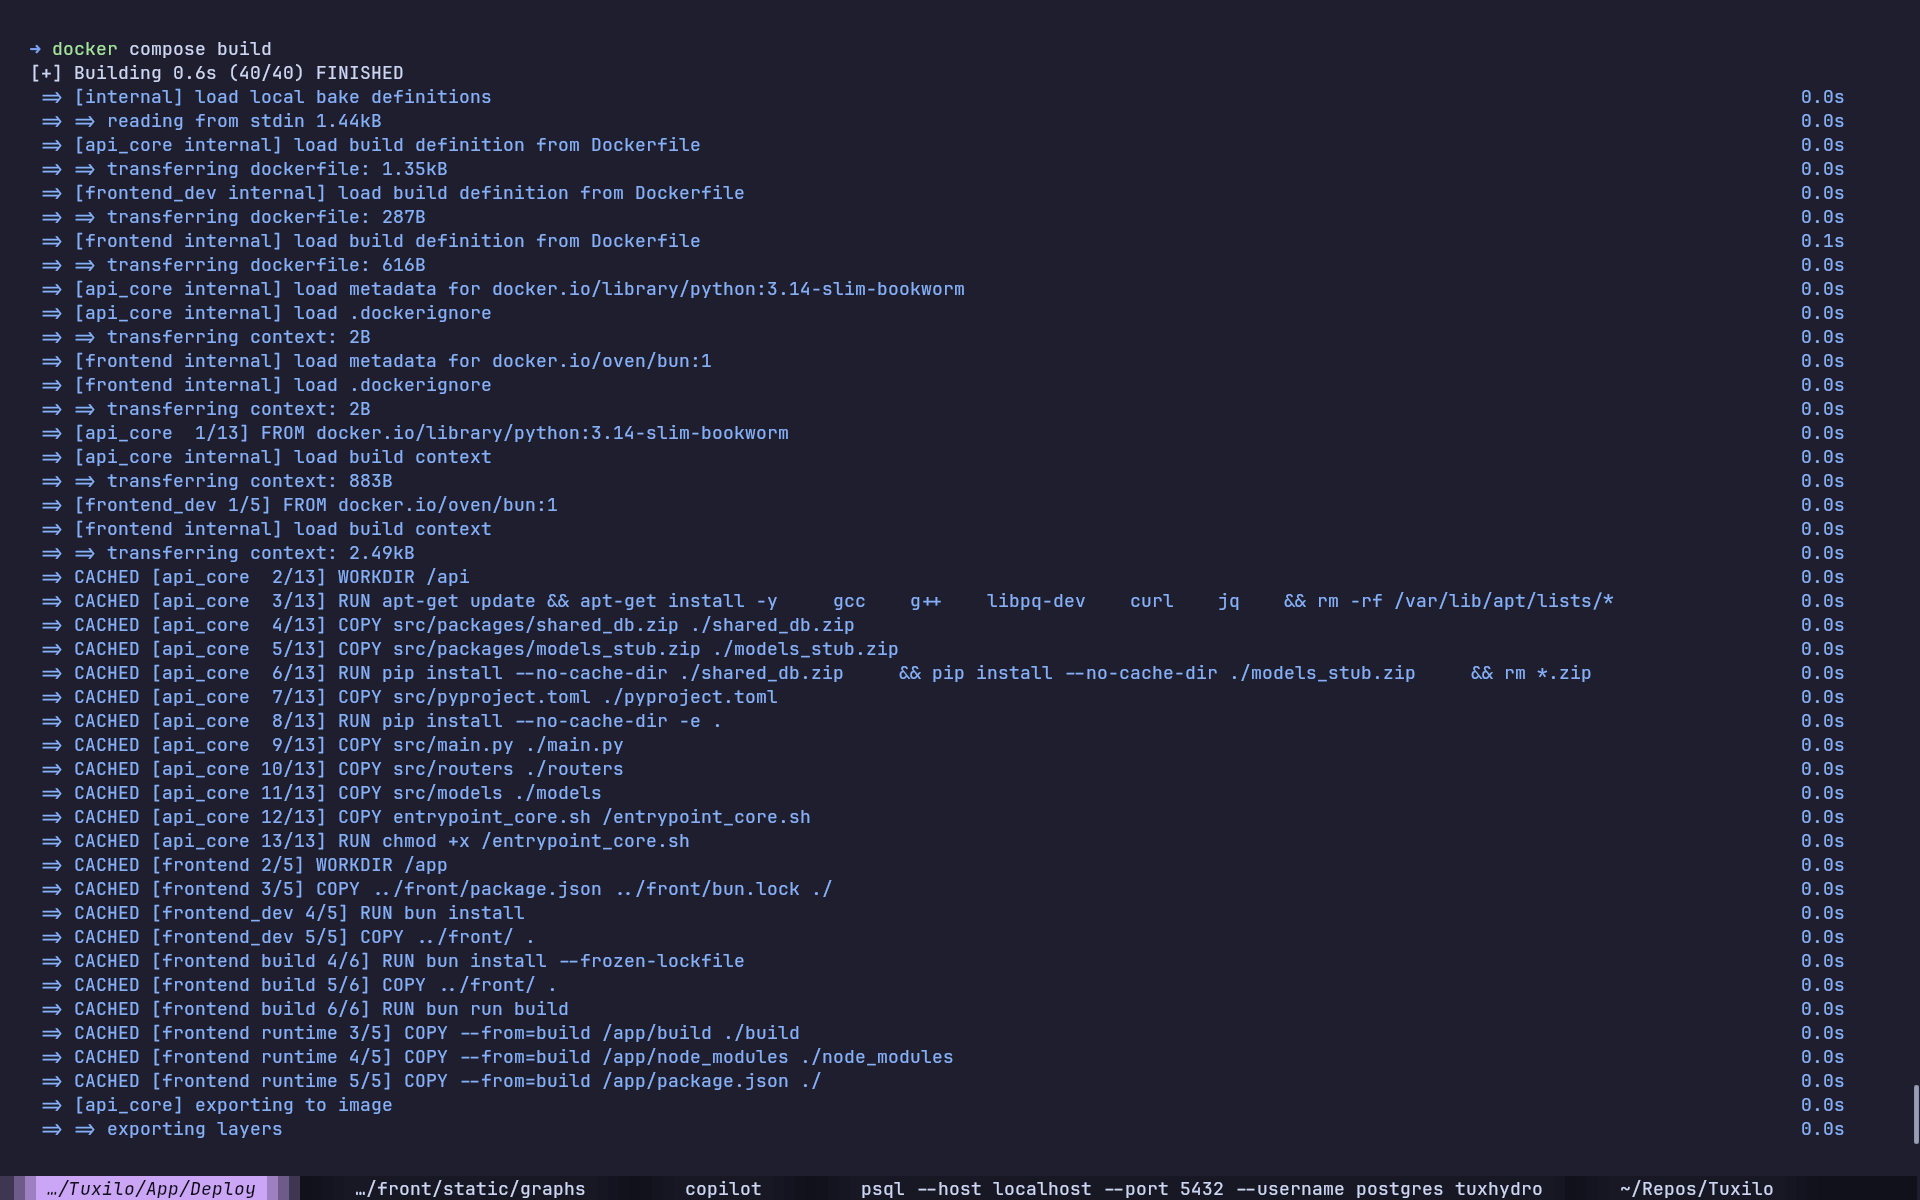
\includegraphics[width=\textwidth]{img/build.png}
  \caption{Proceso terminado del build}
  \label{fig:build}
\end{figure}


\section{Despliegue y ejecución}
\label{sec:chp7-3}

Una vez completada la instalación y configuración, el sistema está listo para su despliegue. Esta sección describe cómo iniciar, detener y gestionar los diferentes servicios.

\subsection{Inicio de servicios}
\label{subsec:chp7-3-1}

Para iniciar todos los servicios del sistema en modo producción, se debe ejecutar:

\begin{lstlisting}[style=bash]
cd App/Deploy
docker compose up -d
\end{lstlisting}

El flag \lstinline[style=bash]|-d| indica que los contenedores se ejecutarán en segundo plano (modo \textit{detached}). Docker Compose iniciará los siguientes servicios en el orden adecuado:

\begin{enumerate}
    \item \textbf{db (gis\_db)}: Base de datos PostgreSQL con extensión PostGIS\cite{postgis}
    \item \textbf{api\_core}: Servidor de API que expone los endpoints de datos
    \item \textbf{frontend}: Aplicación web de visualización
    \item \textbf{frontend\_dev}: Servidor de desarrollo (opcional)
    \item \textbf{nginx}: Servidor web reverse proxy
    \item \textbf{pgadmin}: Interfaz web de administración de base de datos
\end{enumerate}

En la figura~\ref{fig:compose-up} se muestra cómo deberían estar los servicios y la salida del \lstinline[style=bash]|docker compose up -d|.

\begin{figure}[H]
  \centering
  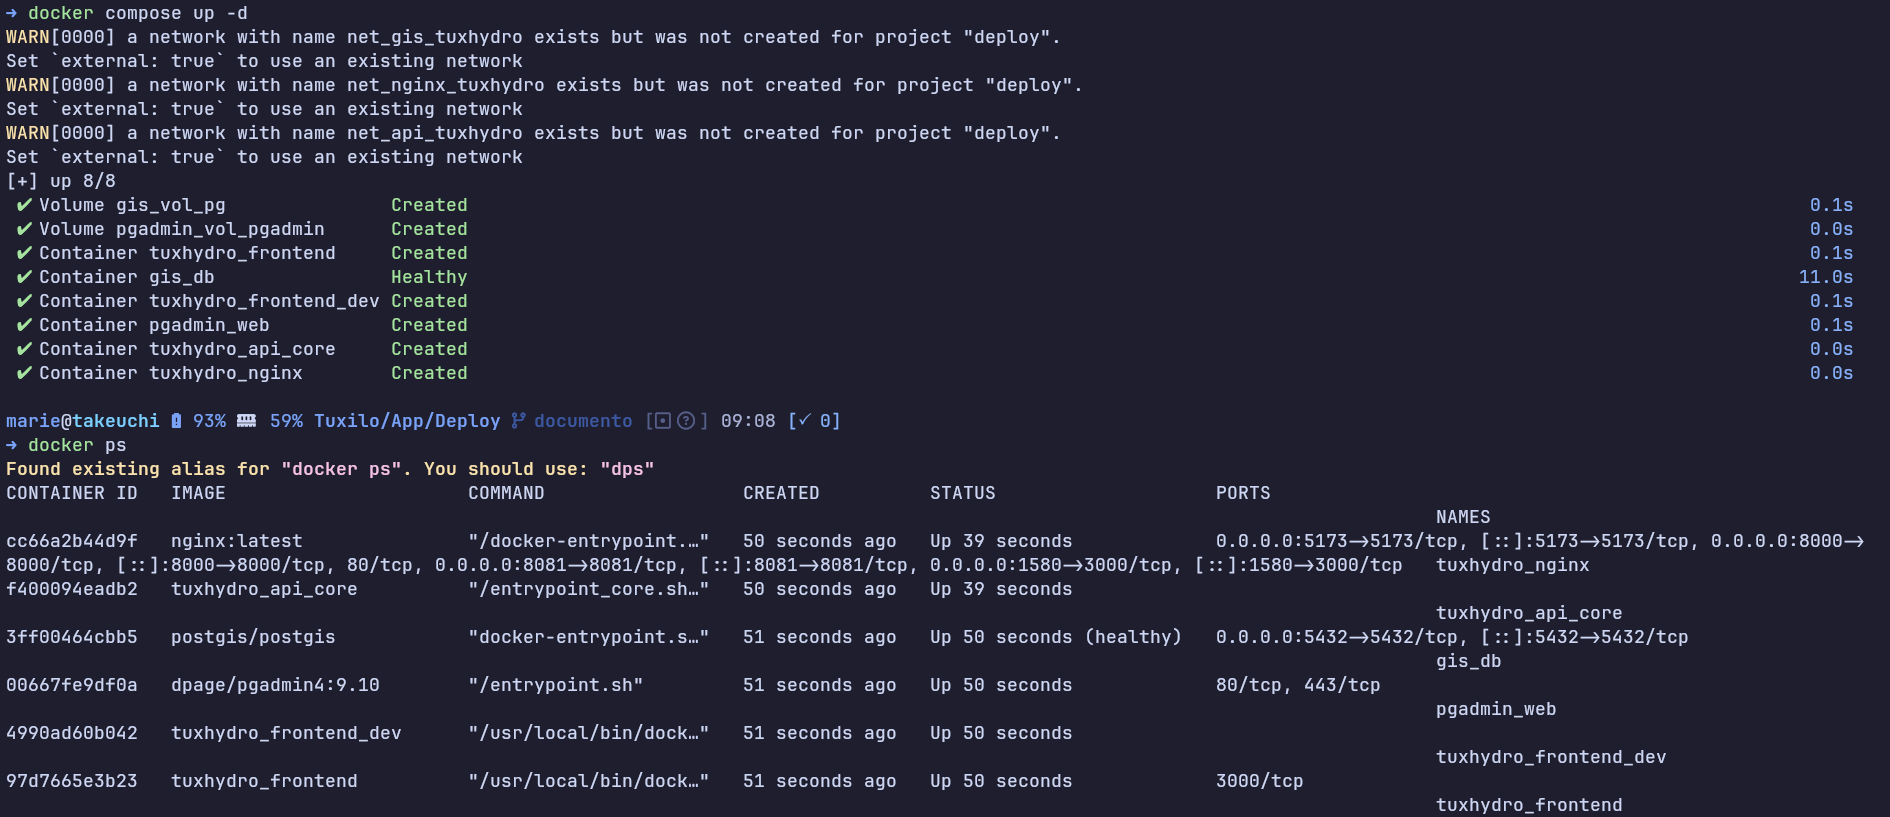
\includegraphics[width=\textwidth]{img/up.png}
  \caption{Servicios corriendo en la maquina local}
  \label{fig:compose-up}
\end{figure}

La primera vez que se ejecuta el sistema, la base de datos se inicializa automáticamente ejecutando los scripts SQL ubicados en \url{scripts/ddl/} y \url{scripts/dml/}, que crean las tablas necesarias y cargan los datos iniciales desde los archivos CSV ubicados en \url{data/}.

\subsection{Verificación del despliegue}
\label{subsec:chp7-3-2}

Para verificar que todos los contenedores se han iniciado correctamente, se puede ejecutar:

\begin{lstlisting}[style=bash]
docker compose ps
\end{lstlisting}

Este comando debe mostrar todos los servicios en estado \lstinline[style=bash]|running| (figura~\ref{fig:compose-up}). En caso de que algún servicio presente errores, se pueden consultar los logs con:

\begin{lstlisting}[style=bash]
docker compose logs nombre_servicio
\end{lstlisting}

Por ejemplo, para ver los logs del API:

\begin{lstlisting}[style=bash]
docker compose logs api_core
\end{lstlisting}

\subsection{Acceso a la aplicación}
\label{subsec:chp7-3-3}

Una vez que todos los servicios estén operativos, se puede acceder a las diferentes interfaces del sistema a través de las siguientes URLs (considerando la configuración por defecto):

\begin{itemize}
    \item \textbf{Aplicación web principal}: \url{http://localhost:1580}
    \item \textbf{Versión de desarrollo}: \url{http://localhost:5173} (con hot-reload)
    \item \textbf{API REST}: \url{http://localhost:8000}
    \item \textbf{Documentación API (Swagger)}: \url{http://localhost:8000/docs}
    \item \textbf{pgAdmin}: \url{http://localhost:8081}
\end{itemize}

El acceso a pgAdmin requiere las credenciales configuradas en el archivo \lstinline[style=bash]|.env|. Una vez autenticado, se puede conectar al servidor de base de datos utilizando el hostname \lstinline[style=bash]|gis_db| (nombre del contenedor dentro de la red Docker).

\subsection{Detención y reinicio de servicios}
\label{subsec:chp7-3-4}

Para detener todos los servicios preservando los datos:

\begin{lstlisting}[style=bash]
docker compose stop
\end{lstlisting}

Para reiniciar los servicios:

\begin{lstlisting}[style=bash]
docker compose start
\end{lstlisting}

Para detener y eliminar los contenedores (manteniendo los volúmenes de datos):

\begin{lstlisting}[style=bash]
docker compose down
\end{lstlisting}

Para eliminar completamente todo, incluyendo volúmenes de datos:

\begin{lstlisting}[style=bash]
docker compose down -v
\end{lstlisting}

\textbf{Advertencia}: El último comando eliminará toda la información de la base de datos. Usar solo cuando se desee reiniciar completamente el sistema.



\section{Recomendaciones para uso institucional}
\label{sec:chp7-6}

Para una implementación exitosa del sistema en un entorno institucional, se presentan las siguientes recomendaciones organizadas por área.

\subsection{Seguridad y acceso}
\label{subsec:chp7-6-1}

\begin{itemize}
    \item \textbf{Autenticación}: Para ambientes de producción, se recomienda implementar un sistema de autenticación y autorización en la API, utilizando tokens JWT o OAuth2
    \item \textbf{HTTPS}: Configurar certificados SSL/TLS para acceso seguro mediante HTTPS, utilizando Let's Encrypt o certificados institucionales
    \item \textbf{Firewall}: Limitar el acceso a los puertos de servicio únicamente desde redes autorizadas
    \item \textbf{Secretos}: Nunca almacenar contraseñas en el control de versiones. Utilizar sistemas de gestión de secretos como HashiCorp Vault o AWS Secrets Manager
    \item \textbf{Actualizaciones}: Mantener actualizadas las imágenes de Docker y las dependencias para corregir vulnerabilidades de seguridad
\end{itemize}

\subsection{Monitoreo y mantenimiento}
\label{subsec:chp7-6-2}

\begin{itemize}
    \item \textbf{Logs centralizados}: Implementar un sistema de agregación de logs como ELK Stack (Elasticsearch, Logstash, Kibana) o Grafana Loki
    \item \textbf{Métricas}: Configurar Prometheus para recolectar métricas de los contenedores y servicios
    \item \textbf{Alertas}: Establecer alertas automáticas para condiciones críticas (caída de servicios, uso excesivo de recursos, errores en la API)
    \item \textbf{Respaldos}: Programar respaldos automáticos de la base de datos PostgreSQL utilizando \lstinline[style=bash]|pg_dump| o soluciones de backup continuo
    \item \textbf{Documentación operativa}: Mantener documentación actualizada de procedimientos operativos, contactos de soporte y planes de contingencia
\end{itemize}

\subsection{Actualización de datos}
\label{subsec:chp7-6-3}

El sistema requiere actualización periódica de los datos para mantener la precisión de las proyecciones:

\begin{itemize}
    \item \textbf{Datos climáticos}: Actualizar mensualmente los índices oceánicos desde las fuentes oficiales (NOAA, CPC)
    \item \textbf{Datos hidrológicos}: Integrar nuevos registros de caudal y precipitación del IDEAM\cite{ideam_dhime_atencionciudadano} y del GRDC\cite{grdc_portal}
    \item \textbf{Recalibración}: Revisar y recalibrar semestralmente los coeficientes de regresión ($a_r$, $b_r$) con los nuevos datos disponibles
    \item \textbf{Validación}: Comparar las proyecciones realizadas con las observaciones reales para evaluar la precisión del modelo
\end{itemize}

Para automatizar la actualización de datos, se puede desarrollar un pipeline ETL (Extract, Transform, Load) utilizando herramientas como Apache Airflow o prefect.


\section{Escalabilidad y extensibilidad}
\label{sec:chp7-7}

El sistema ha sido diseñado con arquitectura modular que facilita su escalabilidad horizontal y vertical, así como su extensión funcional.

\subsection{Escalabilidad horizontal}
\label{subsec:chp7-7-1}

Para soportar mayor carga de usuarios concurrentes, se puede escalar horizontalmente mediante las siguientes estrategias:

\begin{itemize}
    \item \textbf{Múltiples instancias de API}: Utilizar Docker Swarm o Kubernetes para desplegar múltiples réplicas del servicio \lstinline[style=bash]|api_core|
    \item \textbf{Balanceo de carga}: Configurar NGINX o HAProxy como load balancer para distribuir las peticiones entre las instancias
    \item \textbf{Caché distribuida}: Implementar Redis o Memcached para cachear respuestas frecuentes y reducir la carga en la base de datos
    \item \textbf{CDN}: Utilizar una red de distribución de contenidos (CloudFlare, AWS CloudFront) para servir los archivos estáticos del frontend
\end{itemize}

\subsection{Escalabilidad vertical}
\label{subsec:chp7-7-2}

Para manejar consultas más complejas o datasets más grandes:

\begin{itemize}
    \item \textbf{Base de datos}: Incrementar los recursos de la base de datos PostgreSQL (CPU, RAM, SSD) y optimizar las consultas con índices adicionales
    \item \textbf{Particionamiento}: Implementar particionamiento de tablas por fechas para mejorar el rendimiento de consultas temporales
    \item \textbf{Read replicas}: Configurar réplicas de lectura de PostgreSQL para distribuir las consultas de solo lectura
\end{itemize}

\subsection{Extensiones funcionales}
\label{subsec:chp7-7-3}

El sistema puede extenderse para incorporar nuevas funcionalidades:

\begin{itemize}
    \item \textbf{Nuevos índices climáticos}: Integrar índices adicionales como PDO (Pacific Decadal Oscillation), NAO (North Atlantic Oscillation), integrando nuevas columnas en la base de datos y actualizando los modelos predictivos
    \item \textbf{Análisis de series temporales avanzado}: Implementar modelos ARIMA, Prophet o redes neuronales recurrentes (LSTM) para mejorar las proyecciones
    \item \textbf{Alertas automáticas}: Desarrollar un sistema de notificaciones que envíe alertas por correo o SMS cuando se detecten escenarios críticos
    \item \textbf{Dashboard ejecutivo}: Crear visualizaciones adicionales con indicadores clave de desempeño (KPIs) para toma de decisiones gerenciales
    \item \textbf{Integración con otros sistemas}: Conectar con sistemas de generación eléctrica para estimar impactos en la producción de energía
    \item \textbf{Módulo de optimización}: Desarrollar algoritmos de optimización para la gestión óptima de embalses considerando las proyecciones
\end{itemize}

\subsection{Migración a infraestructura en la nube}
\label{subsec:chp7-7-4}

Para organizaciones que prefieran infraestructura en la nube, el sistema puede desplegarse en:

\begin{itemize}
    \item \textbf{AWS}: Utilizando ECS (Elastic Container Service) para los contenedores, RDS para PostgreSQL con PostGIS, y S3 para almacenamiento de datos
    \item \textbf{Google Cloud Platform}: Con Google Kubernetes Engine (GKE), Cloud SQL, y Cloud Storage
    \item \textbf{Azure}: Utilizando Azure Kubernetes Service (AKS), Azure Database for PostgreSQL, y Azure Blob Storage
\end{itemize}

En todos los casos, se recomienda utilizar servicios administrados de base de datos para reducir la carga operativa y aprovechar características como backups automáticos, alta disponibilidad y escalabilidad gestionada.

\section{Solución de problemas comunes}
\label{sec:chp7-8}

Esta sección presenta soluciones a problemas frecuentes durante la instalación y operación del sistema.

\subsection{Error al iniciar la base de datos}
\label{subsec:chp7-8-1}

\textbf{Síntoma}: El contenedor \lstinline[style=bash]|gis_db| no inicia o reinicia constantemente.

\textbf{Posibles causas y soluciones}:

\begin{itemize}
    \item Verificar que el archivo de secreto existe: \lstinline[style=bash]|ls -la App/Secrets/postgres_password|
    \item Revisar los logs del contenedor: \lstinline[style=bash]|docker compose logs db|
    \item Verificar que el puerto 5432 no esté ocupado: \lstinline[style=bash]$netstat -tuln | grep 5432$
    \item Eliminar el volumen y reiniciar: \lstinline[style=bash]|docker compose down -v && docker compose up -d|
\end{itemize}

\subsection{Frontend no carga correctamente}
\label{subsec:chp7-8-2}

\textbf{Síntoma}: La página web no se muestra o aparecen errores en la consola del navegador.

\textbf{Posibles causas y soluciones}:

\begin{itemize}
    \item Verificar que el API está respondiendo: \lstinline[style=bash]|curl http://localhost:8000/docs|
    \item Limpiar la caché del navegador (Ctrl+Shift+Del)
    \item Revisar logs del frontend: \lstinline[style=bash]|docker compose logs frontend|
    \item Reconstruir la imagen del frontend: \lstinline[style=bash]|docker compose build frontend --no-cache|
\end{itemize}

\subsection{Datos no se cargan en la base de datos}
\label{subsec:chp7-8-3}

\textbf{Síntoma}: La aplicación funciona pero no muestra embalses o datos de caudal.

\textbf{Posibles causas y soluciones}:

\begin{itemize}
    \item Verificar que los archivos CSV existen en los directorios esperados (\lstinline[style=bash]|data/Caudal/|, \lstinline[style=bash]|data/Precipitación/|)
    \item Conectar a la base de datos con pgAdmin y verificar que las tablas contienen datos
    \item Revisar logs del proceso de inicialización: \lstinline[style=bash]$docker compose logs db | grep -i error$
    \item Ejecutar manualmente los scripts SQL: conectarse a la base de datos y ejecutar los scripts en orden desde \lstinline[style=bash]|scripts/ddl/| y \lstinline[style=bash]|scripts/dml/|
\end{itemize}

\subsection{Problemas de rendimiento}
\label{subsec:chp7-8-4}

\textbf{Síntoma}: La aplicación responde lentamente o las consultas tardan mucho.

\textbf{Posibles causas y soluciones}:

\begin{itemize}
    \item Incrementar recursos asignados a Docker (Docker Desktop $\rightarrow$ Settings $\rightarrow$ Resources)
    \item Crear índices en la base de datos para las columnas más consultadas
    \item Implementar caché en la API para respuestas frecuentes
    \item Optimizar consultas SQL revisando el plan de ejecución con \lstinline[style=bash]|EXPLAIN ANALYZE|
\end{itemize}

% \section{Consideraciones finales}
% \label{sec:chp7-9}

% La solución desarrollada representa una base sólida para el análisis de la relación entre índices oceánicos y el comportamiento hidrológico de embalses en Colombia. Su arquitectura modular y el uso de tecnologías estándar de la industria facilitan su adopción, mantenimiento y evolución.

% Para maximizar el valor de esta herramienta en un contexto institucional, se recomienda:

% \begin{enumerate}
%     \item Integrarla en los flujos de trabajo existentes de planificación energética
%     \item Establecer protocolos de actualización regular de datos
%     \item Validar continuamente las proyecciones con observaciones reales
%     \item Documentar lecciones aprendidas y casos de uso exitosos
%     \item Contribuir mejoras y extensiones al repositorio público para beneficio de la comunidad
% \end{enumerate}

% El código completo, documentación técnica y datos del proyecto están disponibles en el repositorio \url{https://github.com/GNUTADEO/Tuxilo/} bajo licencias de software libre, promoviendo la transparencia, replicabilidad y colaboración en el análisis hidroclimático nacional.
